\documentclass{article} % For LaTeX2e
\usepackage{nips13submit_e,times}
\usepackage{hyperref}
\usepackage{url}
\usepackage{graphicx}
\usepackage{amsmath}
\usepackage{amsfonts}
%\documentstyle[nips13submit_09,times,art10]{article} % For LaTeX 2.09


\title{Predicting Popularity of YouTube Video}

\author{
Loc Do \\
Heinz College,
Carnegie Mellon University \\
Pittsburgh PA, 15213\\
\texttt{halocd@andrew.cmu.edu} \\
\And
Joseph Richardson \\
School of Computer Science,
Carnegie Mellon University \\
Pittsburgh PA, 15213 \\
\texttt{jmrichar@andrew.cmu.edu} \\
}

\newcommand{\fix}{\marginpar{FIX}}
\newcommand{\new}{\marginpar{NEW}}

\nipsfinalcopy % Uncomment for camera-ready version

\begin{document}

\maketitle

\section{Introduction}
\label{sec:intro}
YouTube is one of the most popular video-sharing online platform in the Internet. It attracts billion of unique user visit monthly and has diverse topics in their video content. YouTube users can earn money from the number of views of their uploaded videos. Hence, understanding the secrets of making a popular YouTube video is essential for people who want to make benefits from the site. There are many factors to determine popularity of a video, but in general we can pin down to have the following two: having good content and good marketing plan. One of the techniques to attract more viewerships is to make the video's "visual appearance" look appealing such as catchy keywords, informative cover picture, etc. Our approach is to utilise a video's metadata to predict their popularity.

The ranking problem (aka. Learning to rank\footnote{http://en.wikipedia.org/wiki/Learning\_to\_rank}) is a typical supervised learning problem of predicting the rank of a set of items regarding to a set of criteria. It has a numerous applications in a broad domains such as web search, multimedia retrieval, recommender systems, etc. Results from these such problems can bring benefits to Internet users such as saving their time by introducing the most relevant products/articles/web pages to their interests. In YouTube context, ranking problems can be raised to recommend most relevant videos to a given video. Another application is to predict the ranking of videos w.r.t to their popularity. This can reveal the most important visual factors in determine popularity of a video.

\textbf{Problem statement.} Given a set of videos, each is associated with a set of bag-of-word and numeric features. A pair of videos is said to have an order on their popularity by comparing their number of views. Video with more viewership is considered to be more popular than the other. Given two videos with their features, the ranking problem here is to construct a model to accurately predict the exact order between the two videos.

\section{Ranking the popularity}
\label{sec:ranking}	
	Our goal is to construct a prediction rule $f$ that can rank the videos w.r.t. their popularity using their meta-data as feature inputs.
	\subsection{Ranking as Logistic Regression}
We can reformulate the ranking prediction problem between two videos as a binary classification problem. To be specific, let $X_i \in \mathbb{R}^D$ and $X_j \in \mathbb{R}^D$ be feature vectors of two video $i$ and $j$ correspondingly. Each video pair $(i, j)$ is associated with a binary label $Y_{ij}$ defined as follows
\begin{equation}
	Y_{ij} = \begin{cases}
			   1, & \text{if } \text{\#\_of\_views\_i} \geq \text{\#\_of\_views\_j} \\
			   0, & \text{otherwise}
			\end{cases} 
\end{equation}	
 We can form a representative vector of the pair $(i, j)$ as follows
\begin{equation}
	\mathcal{X}_{ij} = k (X_i, X_j),
\end{equation}
where $k: (\mathcal{R}^D, \mathcal{R}^D) \rightarrow \mathcal{R}^{D'}$ is a feature transformation function. There are several options for $k$. 
\begin{itemize}
	\item Difference between two feature vectors: $\mathcal{X}_{ij} = X_i - X_j$
	\item Concatenation of two feature vectors:  $\mathcal{X}_{ij} = [X_i, X_j]$ (Matlab notation)
	\item Kernel functions, e.g. $\mathcal{X}_{ij} = || X_i - X_j ||^2$
\end{itemize}
At the moment, we cannot find any theories/signals to indicate which form of $k$ is the most appropriate. For the scope of the project, we choose to represent $X_{ij}$ as difference between $X_i$ and $X_j$, meaning $D = D'$. The kernelized version is left in future work. 

The function form of classifier $P(Y_{ij}|\mathcal{X}_{ij}, \textbf{w})$ as follows
 \begin{equation}
	 P(Y_{ij}=1|\mathcal{X}_{ij}, \textbf{w}) = \frac{1}{1 + \exp ( w_0 + \sum_d w_d \mathcal{X}_{ij}^d )} = \frac{1}{1 + \exp (\textbf{w}^T \mathcal{X}_{ij})}
 \end{equation}
 
The model parameters $\textbf{w} \in \mathbb{R}^D$ can be learnt using MAP.
\begin{align}
	\label{eqn:objFuncLR}
	\hat{\textbf{w}}_{MAP} &= \operatorname*{arg\,max}_{\textbf{w}} \prod_{(i,j)} P(Y_{ij}| \mathcal{X}_{ij}, \textbf{w}) P(\textbf{w}) \hspace{1 cm} \text{($P(\textbf{w}) \sim \mathcal{N} (0, \tau^2 I) $)}\\ \notag
	&= \operatorname*{arg\,max}_{\textbf{w}} \prod_{\{(i,j)|Y_{ij}=1\}} P(Y_{ij}| \mathcal{X}_{ij}, \textbf{w}) P(\textbf{w}) \hspace{1 cm} \text{($Y_{ij} + Y_{ji} = 1, \mathcal{X}_{ij} = - \mathcal{X}_{ji}$)}\\ \notag
	&= \operatorname*{arg\,max}_{\textbf{w}} \sum_{\{(i,j)|Y_{ij}=1\}} ln P(Y_{ij}| \mathcal{X}_{ij}, \textbf{w}) + ln P(\textbf{w}) \\ \notag
	&= \operatorname*{arg\,max}_{\textbf{w}} \sum_{\{(i,j)|Y_{ij}=1\}} ( (1 - Y_{ij})\textbf{w}^T\mathcal{X}_{ij} - ln(1 + \exp(\textbf{w}^T\mathcal{X}_{ij}))) - \lambda_w \|\textbf{w} \|^2_2 = l(\textbf{w})
\end{align}

We can optimise Equation \ref{eqn:objFuncLR} (a concave function) using Gradient Ascent with the following update rule
\begin{equation}
w^{t+1}_d \leftarrow w^t_d + \eta \frac{\partial l(\textbf{w})}{\partial w_d} = w^t_d + \sum_{\{(i,j)|Y_{ij}=1\}} \mathcal{X}_{ij}^d ( (1 - Y_{ij}) - \frac{\exp(\textbf{w}^T\mathcal{X}_{ij})}{1 + \exp(\textbf{w}^T\mathcal{X}_{ij})})  - \lambda_w w_d
\end{equation}

	Another approach to the ranking problem is to predict the number of views for each video and then rank the videos based on predicted values, rather than comparing two videos directly. This approach has two advantages over the above approach of classification. First, it can take into account the magnitude of difference between two videos' viewership. Secondly, we can use it to predict a number of views of a video for a specific time in future given their current status. We treat this problem as an ordinary linear regression problem. 

\subsection{Problem Formulation}
Our linear function assumes that are labels $Y_i$ come from our input $X_i$ plus some noise $\epsilon$:
\begin{equation}
Y_u = X_u \beta + \epsilon,
\end{equation}
where $Y_i$ is the number of views of video $i$, $X_i$ is the associated feature vector. We therefore seek a function of the form
\begin{equation}
f(X) = X \beta
\end{equation}
and attempt to minimize the mean squared error loss function, giving
\begin{equation}
	\hat{\beta} = \operatorname*{arg\,min}_{\textbf{$\beta$}} 1/n (A \beta - Y)^T(A \beta - Y)
\end{equation}
where $A = [X_1 ... X_n]^T$ and $Y = [Y_1 ... Y_n]^T$, n is the number of training data points.

%We anticipated that this method will perform worse than logistic regression at the ranking problem.  However, this method, if successful, would have the added utility of allowing predictions on a video without needing to compare it to another.

In order to solve this problem, we can use either the closed form or Gradient Descent to learn the $\beta$ parameters.  However, since our feature space may be quite large, we opt for the latter.  We therefore initialize $\beta^0$ to 0, and thereafter use the update step
\begin{equation}
\beta^{t+1} = \beta^t - \eta A^T (A \beta^t - Y)
\end{equation}
 
Since our context is a bad conditioning problem, similarly to the Classification approach, we opt to Stochastic Gradient Descent with L2-Regularization. The new update function
	\begin{equation}
		\beta^{t+1} = \beta^t - \eta (x_i (x_i\beta^t - Y_i) + \beta^t)
	\end{equation}

After the learning stage is complete, the predicted ranking can be done as follows
\begin{equation}
\hat{Y}_{uv} = \mathbb{I}(\beta X_u > \beta X_v),
\end{equation}
where $\mathbb{I}$ is the indicator function, return 1 if the expression as argument is true, and 0 otherwise.

\subsection{Comparing Order-of-Magnitude}
\label{sec:orderofmagnitude}
	It is important to decide what we will consider as being "close to correct".  We use least-squared regression, where we minimize the total of the squares of the differences between our prediction and the true value.  However, we must deal with the gigantic variance in our observed data.

	Ideally, we wish to consider orders of magnitude rather than direct counts, and for this we will set our loss function equal to the square of the difference between the log of our prediction and the log of the observed value.  The motivation is that we wish to reflect the human intuition that there is more difference between the popularities of two videos with 10 and 1,000 views (respectively) than between two videos with 1,000,000 and 1,001,000 views.  This will prevent petty variations among the most popular videos from drowning out the differences in all others.

	We therefore deal with the number of views in log scale for the regression (though we also tried running our analysis without using log scale).  One anticipated effect of this is that features will be expected to contribute multiplicatively, rather than additively, to the popularity of a video.

\subsection{Dataset}
	We crawled and extracted our data from YouTube for one month (Oct - Nov, 2015). The crawling strategy is akin to bread-first search. First we initialize the crawler with several random "seed" videos, which mostly are in the \textit{Movie} and \textit{Music} category, and recursively explore all other related videos recommended by YouTube recommendation systems. For each video, we extract all of its metadata such as title, uploader and his number of subscriptions, description, upload date, number of views/likes/dislikes, video length, and a number of other attributes, as well as a list of around 30 videos YouTube recommends as being similar. 

	\subsubsection{Data Statistics}
		Although the crawler was suspended twice due to technical issues and upgrades, we have gathered a sizeable amount of data, with tremendous variation in the observed values:
		
		\begin{itemize}
			\item Number of videos crawled: 1,432,213
			\item Number of uploaders: 628,072
			\item Number of "bag of word" features (extracted from the titles): 2,447,603 entries
			\item Video length: $[1 \ldots 107,373]$ (seconds)
			\item Range of number of day passed since uploaded: $[1 \ldots 3423]$ (days)
			\item Range of number of views: $[7 \ldots 2,104,518,656]$.
			\item Range of number of likes: $[1 \ldots 8,639,650]$.
			\item Range of number of dislikes: $[1 \ldots 4,184,769]$.
		\end{itemize}

		We plot in Figure \ref{fig:histograms} different histograms reflecting characteristics of our data. In the red-colorer histogram, we look for the distributions of videos and their view counts. Interestingly, the distribution is in the shape of Gaussians, instead of following the Power Law distribution as frequently observed in social networks. We guess this observation is due to the way we sampled the data, by following the recommended links. It is intuitive since videos with high view counts are usually recommended together. The Gaussian distribution also encourages us to perform some standardisation on the data, such as subtracting the label to the mean of the Gaussian and predict the left amount. 
		

		\begin{figure}[!h]
			\begin{center}
				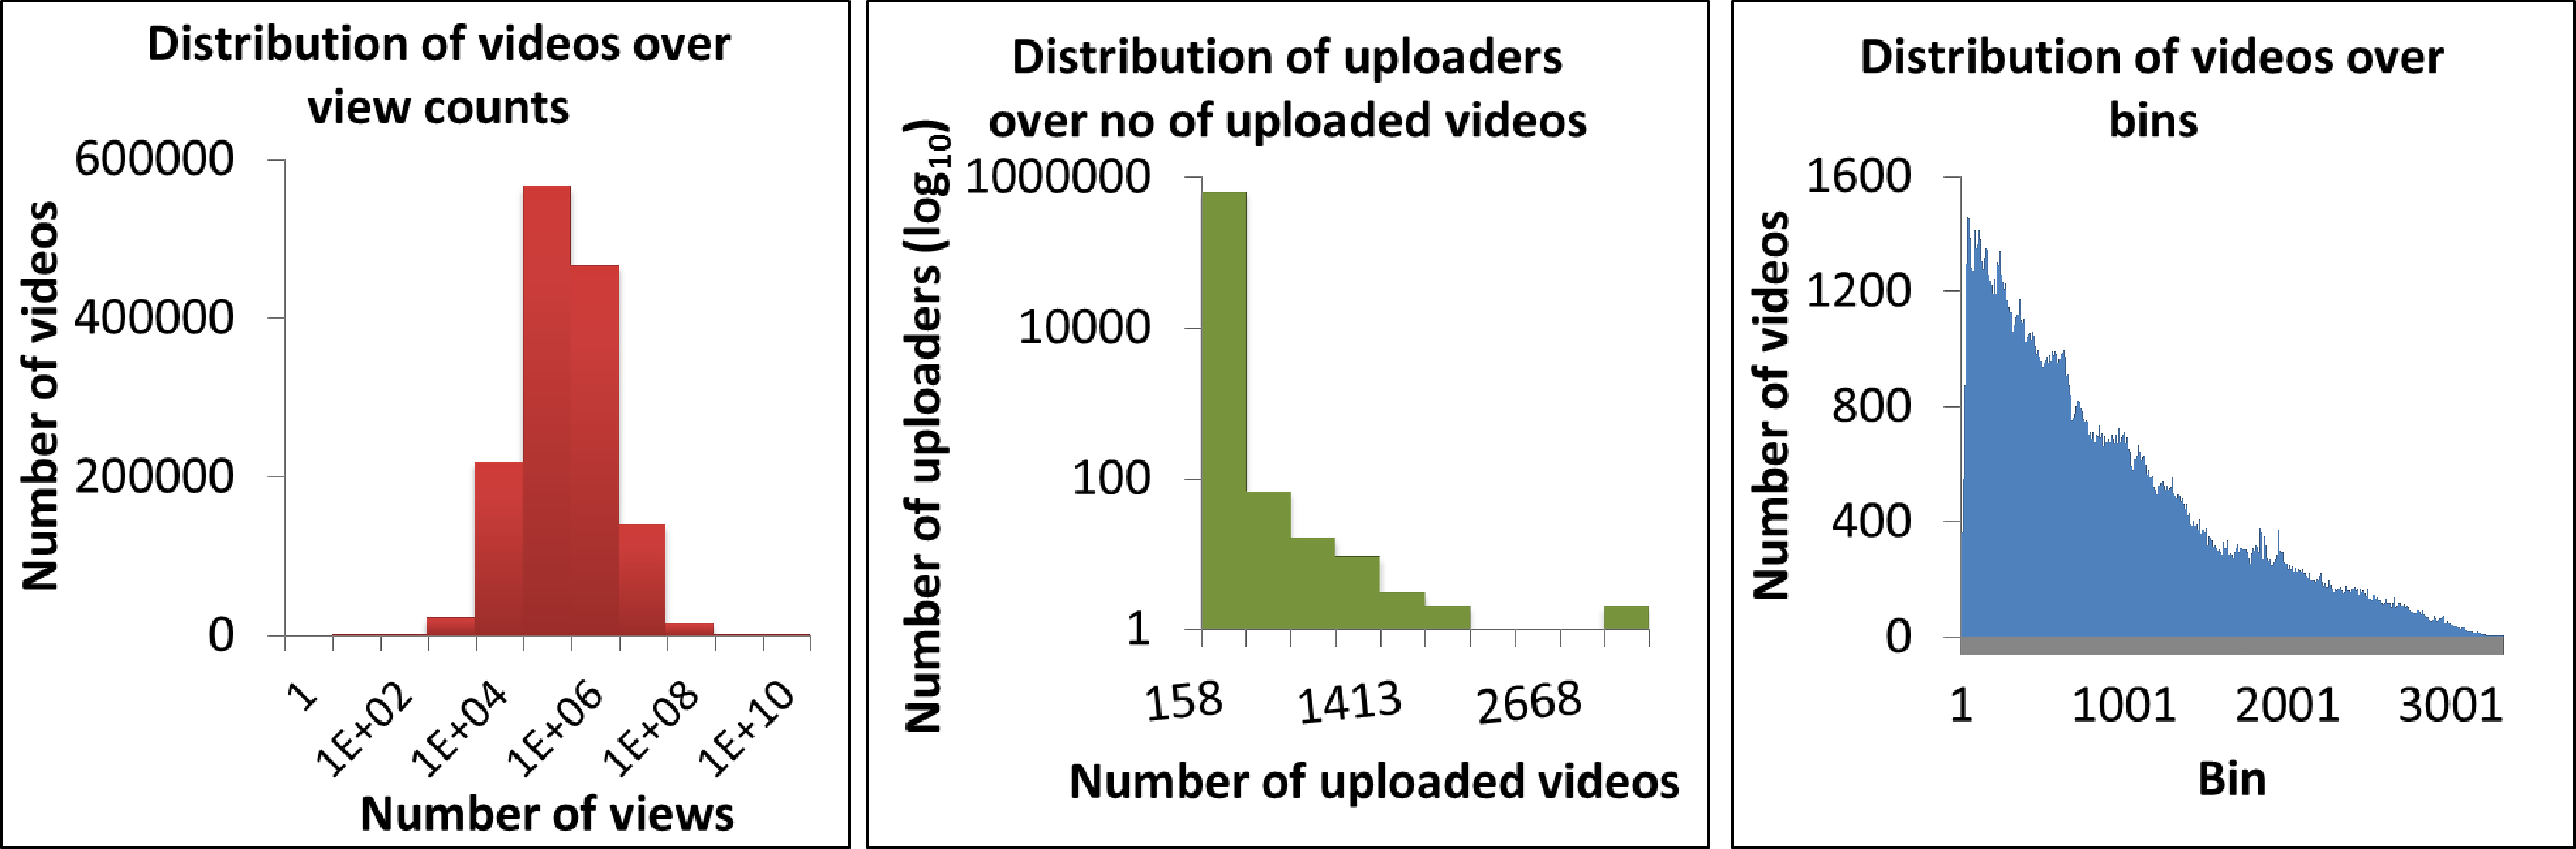
\includegraphics[width=1.0\textwidth,clip]{distributions.pdf}
			\end{center}
			\caption{Red-colored histogram: Distribution of videos over view counts. Blue-colored histogram: Distribution of uploaders over number of uploaded videos. Green-colored histogram: Distribution of number of videos in each bin.}
			\label{fig:histograms}
		\end{figure}
	
		As the statistics show, we have a large magnitude in ranges of number of view, likes and dislikes. This motivates us to do some preprocessing on data, such as feature normalization or data standardization, to ensure the numerical stability and good speed of convergence on the learning algorithm for logistic regression. We discuss more on this step in the Section \ref{sec:orderofmagnitude}.
						
	\subsubsection{Feature extraction}
		In this section we discuss the feature engineering process in the project. First, we build a dictionary mapping the uploader to the number of videos they have uploaded and the total number of views there videos have. We also take care to prevent "cheating":  In order to ensure that our predictor has only such information as would be available before the video's publishing is ever used, we temporarily reduce these number of video-views and the total number of video uploads for the uploader according to the publish date of the video under current consideration.

		We considered many features, which ultimately include:
		\begin{itemize}
			\item
			Features extracted via a bag-of-words model on the title, using TF-IDF.
			\item
			The number of videos uploaded by the uploader prior to the current video's upload date.  Because of our desire for caution against "cheating", we count only those videos that we have crawled.
			\item
			The total number of views for the uploader due to videos released prior to the current video's upload date.  Again, we count only those videos that we have crawled.  This date-conscious counting is particularly important because there are many cases where there is only one video crawled for a given uploader, meaning that this feature would become a nearly perfect predictor.
			\item
			The number of subscribers for the uploader.  We lack sufficient data to know how subscribers changed over time, so we simply had to keep this constant.
			\item
			The runtime of the video, in seconds.
			\item
			The age of the video at the time of crawling, in days.
			\item
			The number of likes/dislikes.  Since these are expected to scale with the number of views, we forbade ourselves from using the number directly, but we did allow certain combinations, such as the log of the like-vs-dislike ratio.
			\item
			Various combinations of the above features (for example, the log of some other feature, or the ratio between two features).
		\end{itemize}
	
\subsection{Evaluation Metrics}
	Normally, a rank correlation \footnote{http://en.wikipedia.org/wiki/Rank\_correlation} is a common metric in ranking problems. Since our problem is re-formulated as a classification and regression problems, we evaluate our methods using corresponding metrics such as Root Mean Square Error (RMSE) for Regression and $F_1$-score and Accuracy for Classification.
	
	\subsubsection{Classification}
	The error matrix (or confusion matrix) is a common way to measure performance of any arbitrary classifiers. Several metrics derived from this matrix are Accuracy, Precision-Recall, $F_1$-score or Receiver Operator Characteristics (ROC). In our work we employ two of them: Accuracy and $F_1$-score \footnote{http://en.wikipedia.org/wiki/F1\_score}.
	
	The accuracy can be equivalently stated as a 0-1 loss function over total number of pairs in testing set.
	\begin{equation}
		0/1_{loss} = \sum_{(u, v)_{test}} \frac{1}{|(u,v)_{test}|} \textbf{1}[\hat{Y}_{uv} - Y_{uv} == 0]
	\end{equation}
	
	\subsubsection{Regression}
	To Joseph: Can you put your least square formula here ? The first few paragraphs in section 4.3.2 can be put here. And show the equations as well.
	
Our problem is a special case of the more general \textbf{Learning to rank} problem, which is widely used in many applications such as Information Retrieval, Data Mining, etc. [1] gives a short survey of state-of-the-art approaches to the problem of ranking documents relevant to user queries. Most of them are implemented in Ranklib\footnote{http://people.cs.umass.edu/~vdang/ranklib.html}.

Another form of the problem is ordinal classification (a.k.a. ordinal regression). There are several approaches, mostly adapted from classification techniques, such as support vectors [2], Gaussian processes [3], etc. Ordinal classification is related to the ranking problem in that both involve predicting the objects' orders, and is, like ranking, a supervised learning tasks. The important difference is in the level of orderings. As [1] discussed, learning to rank cares more about the accurate ordering of objects, while the latter focuses on a categorization that happens to be orderable. 
For example, ordinal regression would try to categorize movies into "one star" through "five stars" categories, but there are no specific rankings between movies with the same number of stars, while the learning to rank algorithm has an absolute ordering between all members.

\section{Conclusion}
\label{sec:conclusion}

	\subsection{To-do list}
	There is one additional piece of information that we decided our crawler should collect, which still needs to be added: the number of subscribers for each user.  Since this was not needed for our original proposal, we will need to go back and gather this information, which may take some time considering the vast quantity of videos crawled.

	\subsection{Stretch Goals}
	We certainly hope to attempt increasingly sophisticated learning techniques to reduce our loss as much as possible.  Time allowing, there are also other interesting results we can persue.  Chief among these in our mind is to make more time-dependent predictions.  It may be, for example, that video A is very popular at first, but that video B maintains it's popularity better over time, eventually overtaking video A in terms of the numbers of views and of likes.

		 
	%\subsection{First Steps Taken}
	%The data gathering required significant time, and is a big part of the project, but apart from this we had to change most of our plans regarding first steps.  Therefore, what we will present in this report is the results of our first attempt to predict the popularity of a video.  For this, we have considered the data from just five days of crawling, and we have reduced the number of fields considered to the title, uploader, video length, and upload date.  We consider only the number-predicting version, not the direct-comparison-prediction version.

	%\subsection{Technique Details}
	%We perform  a linear regression on the log of the number of views ("Y") and some features extracted from our video data ("X"), to find the best $\beta$ for $Y  = \beta * X$.  We also use the log of the number of views as our loss function, rather than using the number of views directly.

	%We then randomly select 80\% of our data for training, and reserve the other 20\% for testing.  Once the training is finished, we run the other 20\% of our data into the trained model, and consider how much loss was observed.

\subsubsection*{Acknowledgments}

Our sincere thanks to Anthony for his patience and value inputs to improve our project.

\small{
[1] Hang, L. I. "A short introduction to learning to rank." IEICE TRANSACTIONS on Information and Systems 94.10 (2011): 1854-1862.

[2] Herbrich, Ralf, Thore Graepel, and Klaus Obermayer. "Support vector learning for ordinal regression." (1999): 97-102.

[3] Chu, Wei, and Zoubin Ghahramani. "Gaussian processes for ordinal regression." Journal of Machine Learning Research. 2005.

[4] Dietterich, Thomas G. "Ensemble methods in machine learning." Multiple classifier systems. Springer Berlin Heidelberg, 2000. 1-15.
}


\end{document}
